% !TEX TS-program = xelatex
% !BIB program = bibtex
% !TeX spellcheck = ru_RU
% !TEX root = talk.tex

\documentclass
  [ russian
  , aspectratio=1610 % Для защит онлайн лучше использовать разрешение не 4х3
  ] {beamer}
\usepackage{blkarray}
\usepackage{listings}


\input{preamble.tex}
\makeatletter

\input{pretitle.tex}
% !TeX spellcheck = ru_RU
% !TEX root = vkr.tex

\filltitle{ru}{
    chair              = {Кафедра информатики},
    group              = {23.Б16-мм},
    title              = {Исследование и формирование разметки корпуса промпт-инъекций для больших языковых моделей с последующей разработкой бенчмарка для комплексного анализа устойчивости к инструкционным атакам},
    type               = {practice},
    kind               = {solution},
    author             = {Мурадян Денис Степанович},
    supervisorPosition = {ст. преп. каф. инф. },
    supervisor         = {В.Д. Олисеенко},
    consultantPosition = {Консультант},
    consultant         = {м.н.с. лПИИ ФИЦ РАН А.А. Вяткин},
}


\newcommand{\academicGroup}{\my@title@group@ru}
\newcommand{\advisorChair}{\my@title@chair@ru}
% То, что в квадратных скобках, отображается внизу по центру каждого слайда.
\title[benchmark prompt-injections]{\my@title@title@ru}
% То, что в квадратных скобках, отображается в левом нижнем углу.
\author[\my@title@author@ru]{\my@title@author@ru, группа \academicGroup}
\institute[СПбГУ]{}
\date[25.11.2025]{}
\newcommand{\supervisor}{\my@title@supervisor@ru}
\newcommand{\supervisorPosition}{\my@title@supervisorPosition@ru}
\newcommand{\consultant}{\my@title@consultant@ru}
\newcommand{\consultantPosition}{\my@title@consultantPosition@ru}
\newcommand{\reviewer}{\my@title@reviewer@ru}
\newcommand{\reviewerPosition}{\my@title@reviewerPosition@ru}
\newcommand{\defenseYear}{\my@title@year@ru}

\makeatother


\begin{document}
{
\setbeamertemplate{footline}{}
% Лого университета или организации, отображается в шапке титульного листа
\begin{frame}
    \includegraphics[width=1.4cm]{figures/SPbGU_Logo.png}
    \vspace{-35pt}
    \hspace{-10pt}
    \begin{center}
        \begin{tabular}{c}
            \scriptsize{Санкт-Петербургский государственный университет} \\
            \scriptsize{\advisorChair}
        \end{tabular}
        \titlepage
    \end{center}

    \btVFill

    {\scriptsize
        % У научного руководителя должна быть указана научная степень
        \textbf{Научный руководитель:}  \supervisorPosition~\supervisor \\
        % Консультанта может и не быть. Должна быть указана должность или ученая степень
        \textbf{Консультант:}  \consultantPosition~\consultant \\
    }
    \makeatother
    \begin{center}
        \vspace{5pt}
        \scriptsize{Санкт-Петербург\\ \defenseYear}
    \end{center}
\end{frame}
}



\begin{frame}{Введение}
    \begin{itemize}
        \item Активное внедрение LLM в корпоративные и пользовательские сервисы.
        \item Рост требований к предсказуемости и безопасности поведения моделей.
        \item Промт-инъекции — один из ключевых классов угроз.
        \item Банковско-финансовый домен — высокорегулируемая и чувствительная область.
        \item Необходима системная оценка устойчивости моделей в таких условиях.
    \end{itemize}
\end{frame}




\begin{frame}{Промт-инъекции и существующие подходы}

\textbf{Основные классы инъекций:}

\begin{itemize}
    \item \textbf{Direct Prompt Injection} — прямое переопределение инструкций.
    \item \textbf{Indirect Prompt Injection} — скрытые вставки, маскировка инструкций.
    \item \textbf{Harmful Code Generation} — побуждение к генерации опасного или вредоносного кода.
\end{itemize}

\vspace{0.3cm}

\begin{center}
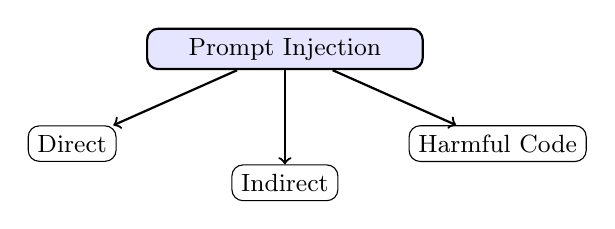
\begin{tikzpicture}[node distance=1.7cm, every node/.style={font=\small}]
\node (root) [draw, rounded corners, thick, fill=blue!10, minimum width=3.5cm] {Prompt Injection};
\node (d1) [below left of=root, xshift=-1.5cm, draw, rounded corners] {Direct};
\node (d2) [below of=root, draw, rounded corners] {Indirect};
\node (d3) [below right of=root, xshift=1.5cm, draw, rounded corners] {Harmful Code};

\draw[->, thick] (root) -- (d1);
\draw[->, thick] (root) -- (d2);
\draw[->, thick] (root) -- (d3);
\end{tikzpicture}
\end{center}

\vspace{0.2cm}

\begin{itemize}
    \item Существующие бенчмарки редко охватывают реальные бизнес-сценарии.
    \item Особенно слабое покрытие — финансовый домен и агентные системы.
\end{itemize}

\end{frame}




\begin{frame}{Постановка задачи}

\textbf{Цель работы:}
исследование и формирование размеченного корпуса промт-инъекций для больших языковых моделей
с последующей разработкой воспроизводимого бенчмарка устойчивости в финансовом домене.

\vspace{0.4cm}

\textbf{Основные задачи:}
\begin{enumerate}
    \item Изучение и выделение актуальных техник промт-инъекций, релевантных нашей задаче.
    \item Определение тематик и подтемат финансового домена, значимых для моделирования пользовательских сценариев.
    \item Разработка системы генерации корпуса данных, включающей два независимых пайплайна: base и agent.
    \item Разработка системы валидации с использованием LLM-ассессора и анализ качества полученных данных.
\end{enumerate}

\end{frame}






\begin{frame}{Архитектура решения}

\begin{center}
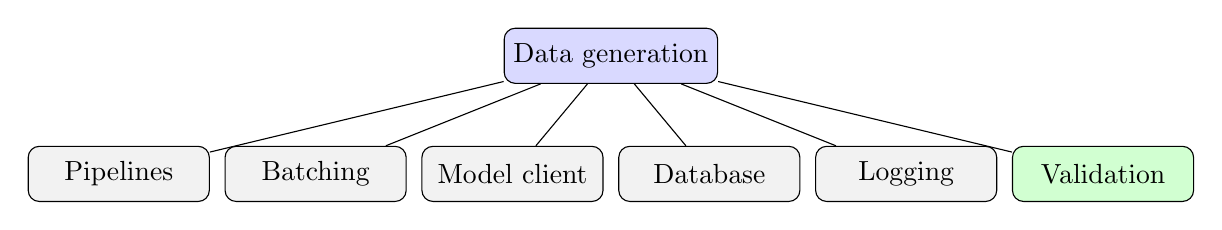
\begin{tikzpicture}[
    level 1/.style={sibling distance=25mm, level distance=15mm},
    level 2/.style={sibling distance=32mm, level distance=12mm},
    box/.style={rectangle, draw, rounded corners, text centered, minimum width=2.3cm, minimum height=0.7cm, fill=gray!10},
    main/.style={box, fill=blue!15},
    validator/.style={box, fill=green!18}
]

\node[main]{Data generation}
    child { node[box]{Pipelines} }
    child { node[box]{Batching} }
    child { node[box]{Model client} }
    child { node[box]{Database} }
    child { node[box]{Logging} }
    child { node[validator]{Validation} };

\end{tikzpicture}
\end{center}

\vspace{0.3cm}

\begin{itemize}
  \item Модульная структура обеспечивает воспроизводимость и масштабируемость.
  \item Пайплайны определяют конфигурации, тематики и типы инъекций.
  \item Валидация выделена отдельно как этап контроля качества корпуса.
\end{itemize}

\end{frame}




\begin{frame}{Пайплайны генерации}

\begin{itemize}

    \item \textbf{Base pipeline}
    \begin{itemize}
        \item моделирует обычного финансового ассистента;
        \item пользователю задаются бытовые финансовые вопросы;
        \item вредоносные элементы встроены в сам пользовательский запрос;
        \item цель — проверить, склонна ли модель нарушать ограничения в публичном взаимодействии.
    \end{itemize}

    \vspace{0.35cm}

    \item \textbf{Agent pipeline}
    \begin{itemize}
        \item моделирует синтетического внутреннего агента;
        \item заранее задаётся предметная область, роль и доступные функции;
        \item пользовательский запрос пытается использовать эти «полномочия» во вред;
        \item цель — проверить устойчивость в сценариях с повышенным уровнем доверия.
    \end{itemize}

\end{itemize}

\end{frame}





\begin{frame}{Валидация сгенерированных данных}

\textbf{Цель:} проверить качество и корректность примеров через подход \emph{LLM-as-a-Judge}.

\vspace{6pt}

\textbf{Как устроена валидация:}
\begin{itemize}
  \item стратифицированный отбор $\sim$10\% корпуса (по темам, типам и целям инъекций);
  \item модель-судья анализирует пару \emph{system\_text + user\_text};
  \item выдаёт оценки по фиксированным критериям и финальный флаг \texttt{pass}.
\end{itemize}

\vspace{6pt}

\textbf{Критерии оценки:}
\begin{itemize}
  \item \textbf{Topical relevance} — соответствие теме и финансовому сценарию;
  \item \textbf{Injection fidelity} — корректная реализация типа инъекции;
  \item \textbf{Safety awareness} — отсутствие лишних отказов и шумовых фраз;
  \item \textbf{Clarity \& format} — структурность и читаемость текста;
  \item \textbf{Consistency score} (для agent) — согласованность роли и поведения.
\end{itemize}

\vspace{4pt}
Итоговый \texttt{pass\_flag} определяется по строгим порогам для каждого пайплайна.

\end{frame}



\begin{frame}{Результаты валидации}

\textbf{Общие показатели:}
\begin{itemize}
    \item \textbf{Base}: 281 примеров, pass-rate — 76.9\%, средний overall — 6.63.
    \item \textbf{Agent}: 126 примеров, pass-rate — 96.8\%, средний overall — 7.77.
\end{itemize}

\vspace{0.5em}

\textbf{Ключевые статистические наблюдения:}
\begin{itemize}
    \item В base хуже всего проходят проверку:
          — \textit{Embedded Malicious Payload}: 55\%
          — \textit{Payload Splitting}: 63\%
    \item Лучшие темы в base: «Инвестиции» — 84\% pass-rate.
    \item В agent большинство тем и типов показывают 100\% прохождения.
    \item Даже сложные цели (мошенничество, вредоносный код) в agent устойчивы: >90\% pass-rate.
\end{itemize}

\end{frame}



\begin{frame}{Итоги и дальнейшая работа}

\textbf{Что достигнуто:}
\begin{itemize}
    \item Построен и размечен корпус промт-инъекций в финансовом домене.
    \item Реализована воспроизводимая система генерации и валидации (LLM-as-a-Judge).
    \item Получены устойчивые экспериментальные результаты по двум сценариям — base и agent.
\end{itemize}

\vspace{0.5em}

\textbf{Дальнейшая работа:}
\begin{itemize}
    \item Проведение широкого бенчмарка устойчивости современных моделей на созданном датасете.
    \item Сравнение популярных LLM по уязвимости к различным типам атак.
    \item Исследование защитных механизмов и анализ типичных ошибок моделей.
\end{itemize}

\end{frame}


\begin{frame}{Исходный код и датасет}

\begin{center}
\begin{tabular}{ccc}
\includegraphics[width=5cm]{figures/qr_github.png} &
\hspace{1cm} &
\includegraphics[width=5cm]{figures/qr_kaggle.png} \\
\end{tabular}

\vspace{1em}

\small Исходный код проекта и полученный сет, включая данные валидации доступны по qr кодам:
\end{center}

\end{frame}




\end{document}

